\documentclass{../HM}
\newcommand\course{HM 2}
\newcommand\hwnumber{9}
\usepackage{gauss}
\usepackage{tikz}
\usepackage{pgfplots}

\begin{document}
	\begin{enumerate}
		\item [9.2] In den vier Ecken einer quadratischen Schachtel der Seitenlänge 2 sitzen vier Ameisen, von denen jede in die jeweils im Gegen-Uhrzeigersinn nächste verliebt ist, und daher zu ihr gelangen möchte. Die Ameisen laufen gleichzeitig mit konstanter Geschwindigkeit los, und zwar jeweils auf die von ihr Geliebte zu.
		\begin{enumerate}
			\item Stelle ein lineares System von Differentialgleichungen für die Bahn der Ameisen auf.
			\begin{eqnn}
				\eqntext{Position der Ameise 1:}
				\eqnf{A_1}{\m{x_{11}, x_{12}}}
				\eqntext{Konstante Geschwindigkeit der Ameise 1:}
				\eqnf{v_1}{\frac{A_2-A_1}{|A_2-A_1|}v}
				\eqn{v_1}{\frac{\m{x_{21}\\x_{22}}-\m{x_{11}\\x{12}}}{\left|\m{x_{21}\\x_{22}}-\m{x_{11}\\x{12}}\right|}v}
				\eqntext{$A_2 = A_1$ um 90° rotiert $\Rightarrow \m{x_{21}\\x_{22}}=\m{-x_{12}\\x_{11}}$:}
				\eqn[][\Rightarrow]{v_1}{\frac{\m{-x_{11}-x_{12}\\x_{11}-x_{12}}}{\left|\m{-x_{11}-x_{12}\\x_{11}-x_{12}}\right|}v}
				\eqn[][\Rightarrow]{y}{\m{-1&-1\\1&-1}y\frac{v}{\sqrt{2(x_{11}^2+x_{12}^2)}}}
			\end{eqnn}
			
			\item Bestimme die Bahnkurve der bei $(1,1)$ startenden Ameise.\\\\
			Da sich die Bahnkurve der Ameise durch ihre Geschwindigkeit zum Zeitpunkt $t$ nicht verändert, die Länge des Geschwindigkeitsvektors keinen Einfluss auf die Bahnkurve besitzt, kann der Faktor der Geschwindigkeitsbegrenzung $\frac{v}{\sqrt{2(x_{11}^2+x_{12}^2)}}\to 1$ geändert werden. 
			\begin{eqnn}
				\eqntext{Eigenwerte und Eigenvektoren bestimmen:}
				\eqn{P_\lambda(A)}{\md{-1-\lambda&-1\\-1&1-\lambda}}
				\eqnf{}{(-1-\lambda)^2+1}
				\eqn{\lambda}{\pm i-1}
				\eqnspace
				\eqn[][\Rightarrow]{\lambda_1}{-1-i,}
				\eqnf{\lambda_2}{-1+i}
				\eqnspace
				\eqn[$v_1$][\Leftarrow]{0}{\m{i&-1\\1&i}[\add[\cdot i][+]{0}{1}]}
				\eqn{0}{\m{i&-1\\0&0}}
				\eqn[][\Rightarrow]{v_1}{\m{-i\\1}}
				\eqnspace
				\eqn[$v_2$][\Leftarrow]{0}{\m{-i&-1\\1&-i}[\add[\cdot(-i)][+]{0}{1}]}
				\eqn{0}{\m{-i&-1\\0&0}}
				\eqn[][\Rightarrow]{v_2}{\m{i\\1}}
				\eqnspace
				\eqn[][\Rightarrow]{y^1}{e^{-(1+i)t}\m{-i\\1},}
				\eqnf{y^2}{e^{(-1+i)t}\m{i\\1}}
				\eqn[][\Rightarrow]{y}{y^1c_1+y^2c_2}
			\end{eqnn}
			\begin{eqnn}
				\eqntext{Anfangswert $y(0)=\m{1\\1}$ einsetzen:}
				\eqn[][\Rightarrow]{\m{-i\\1}c_1+\m{i\\1}c_2}{\m{1\\1}}
				\eqn{\m{-i&i\\1&1}[\add[\cdot(-i)][+]{0}{1}]c}{\m{1\\1}[\add[\cdot(-i)][+]{0}{1}]}
				\eqn{\m{-i&i\\0&2}c}{\m{1\\1-i}}
				\eqn[][\Rightarrow]{c_2}{\frac{1}{2}(1-i)}
				\eqn[][\Rightarrow]{c_1}{\frac{1}{2}(1+i)}
				\eqnspace
				\eqn[][\Rightarrow]{y}{\frac{1}{2}\left((1+i)e^{-(1+i)t}\m{-i\\1}+(1-i)e^{(-1+i)t}\m{i\\1}\right)}
			\end{eqnn}
			\begin{tikzpicture}[remember picture,overlay]
			    \node[xshift=-15mm,yshift=-40mm,anchor=north east] at (current page.north east){
				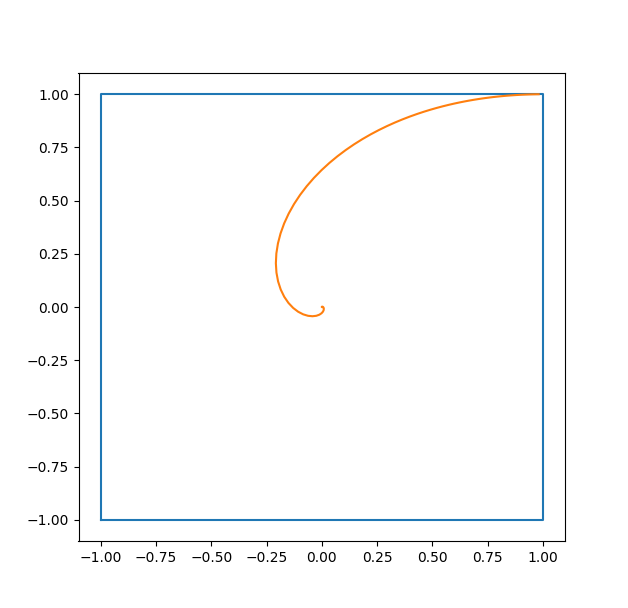
\includegraphics[width=0.4\textwidth]{9.2.png}};
			\end{tikzpicture}
		\end{enumerate}
		
		\item [9.3] Löse das Anfangswertproblem
		$$\begin{cases}
			\dot{y_1}=3y_1+8y_2,&y_1(0)=6,\\
			\dot{y_2}=y_1+y_2+4e^t,&y_2(0)=2.
		\end{cases}$$
		\begin{eqnn}
			\eqn[][\Rightarrow]{\dot{y}}{\m{3&8\\1&1}y+e^t\m{0\\4}}
			\eqntext{Das homogene System lösen:}
			\eqnf{\dot{y}}{\m{3&8\\1&1}y}
			\eqntext{Eigenwerte und Eigenvektoren von $A$ berechnen:}
			\eqnf{P_\lambda(A)}{\md{3-\lambda &8\\1&1-\lambda}}
			\eqn{}{(3-\lambda)(1-\lambda)-8}
			\eqn{0}{\lambda^2-4\lambda+5}
			\eqnspace
			\eqn{\lambda}{2\pm 3}
			\eqn[][\Rightarrow]{\lambda_1}{-1,}
			\eqnf{\lambda_2}{5}
			\eqnspace
			\eqn[$v_1$][\Leftarrow]{0}{\m{4&8\\1&2}[\add[\cdot(-\tfrac{1}{2})][+]{0}{1}]}
			\eqn{0}{\m{4&8\\0&0}}
			\eqn[][\Rightarrow]{v_1}{\m{-2\\1}}
			\eqnspace
			\eqn[$v_2$][\Leftarrow]{0}{\m{-2&8\\1&-4}[\add[\cdot\tfrac{1}{2}][+]{0}{1}]}
			\eqn{0}{\m{-2&8\\0&0}}
			\eqn[][\Rightarrow]{v_2}{\m{4\\1}}
			\eqnspace
			\eqntext{Lösungsbasis der homogenen Differentialgleichung:}
			\eqn[][\Rightarrow]{y^1(t)}{e^{-t}\m{-2\\1},}
			\eqn{y^2(t)}{e^{5t}\m{4\\1}}
			\eqnspace
			\eqntext{Eine spezielle Lösung finden:}
			\eqnf[(I)]{y(t)}{e^tw}[ableiten]
			\eqn[][\Rightarrow]{\dot{y}(t)}{e^tw}
			\geqn[][\Rightarrow]{e^tw}{\feq}{\m{3&8\\1&1}y+e^t\m{0\\4}}
			\eqntext{I einsetzen und kürzen:}
			\eqn{w}{\m{3&8\\1&1}w+\m{0\\4}}[$-\m{3&8\\1&1}w$]
			\eqn{\m{-2&-8\\-1&0}w}{\m{0\\4}}
			\eqn[][\Rightarrow]{w}{\m{-4\\1}}
			\eqn[][\Rightarrow]{y^3}{e^t\m{-4\\1}}
			\eqnspace
			\eqn[][\Rightarrow]{y}{y^1c_1+y^2c_2+y^3}
			\eqntext{Bedingung $y(0)=\m{6\\2}$ einsetzen:}
			\eqnf{\m{-2&4\\1&1}c}{\m{10\\1}}
			\eqn{\m{-2&4\\0&3}c}{\m{10\\6}}
			\eqn[][\Rightarrow]{c}{\m{-1\\2}}
			\eqnspace
			\eqn[][\Rightarrow]{y(t)}{-e^{-t}\m{-2\\1}+2e^{5t}\m{4\\1}+e^t\m{-4\\1}}
		\end{eqnn}		
		
		\item [9.4] Bestimme eine Lösungsbasis der \textit{Bessel'schen Differentialgleichung der Ordnung} $p=\frac{1}{2}$,
		$$y''+\frac{1}{x}y'+(1-\frac{1}{4x^2})y=0$$,\\
		durch die Substitution $z=y\cdot\sqrt{x}$.
		
		\begin{eqnn}
			\eqn[][]{y}{zx^-\frac{1}{2}}
			\eqn{y'}{z'x^{-\frac{1}{2}}-\frac{z}{2}x^{-\frac{3}{2
			}}}
			\eqn{y''}{z''x^{-\frac{1}{2}}-z'x^{-\frac{3}{2}}+\frac{3}{4}zx^{-\frac{5}{2}}}
			\eqntext{Einsetzen in (1)}
			\eqntext{$\Rightarrow z''x^{-\frac{1}{2}}-z'x^{-\frac{3}{2}}+z'x^{-\frac{3}{2}}+\frac{3}{4}zx^{-\frac{5}{2}}-\frac{1}{2}zx^{-\frac{5}{2}}-\frac{1}{4}zx^{-\frac{5}{2}}+zx^{-\frac{1}{2}}$}
			\eqn{z''+ z}{0}
			\eqnspace
			\eqnf{p(\lambda)}{\lambda^2+1=0}
			\eqn[][\Rightarrow]{\lambda}{\pm i}
			\eqn[][\Rightarrow]{z}{c_1\cos+c_2\sin}
			\eqn[][\Rightarrow]{y}{\frac{c_1\cos+c_2\sin}{\sqrt{x}}}
		\end{eqnn}
		
		\item [9.5] Betrachtet wird die Differentialgleichung
		$$\text{(1): }y'''-3y'+2y=9e^x$$.\\
		
		\begin{enumerate}
			\item Bestimme eine Lösungsbasis für die zugehörige homogene Differentialgleichung.
			
			\begin{eqnn}
				\eqn[][]{p(\lambda)}{\lambda^3-3\lambda+2}
				\eqn[][\Rightarrow]{0}{(\lambda-1)^2(\lambda+2)}
				\eqntext{Lösung raten mit hilfe vom Satz über rationale Nullstellen}
				\eqn[][\Rightarrow]{\lambda_1}{1}
				\eqn{0}{\lambda^3-3\lambda+2}[($\lambda-1$)]
				\eqn{0}{\lambda^2+\lambda-2}
				\eqn{0}{(\lambda-1)(\lambda+2)}
				\eqnspace
				\eqntext{$\Rightarrow$ $\lambda_1=1$, $\lambda_2=1$, $\lambda_3=-2$}
				\eqn[][\Rightarrow]{y_H}{c_1e^t+c_2te^t+c_3e^{-2}}
			\end{eqnn}
			\item Finde eine spezielle Lösung durch den Ansatz $y(x)=cx^2e^x$.
				\begin{eqnn}
					\eqn[][\Rightarrow]{y_p}{cx^2e^x}
					\eqn[][\Rightarrow]{y_p'}{ce^x(2x+x^2)}
					\eqn[][\Rightarrow]{y_p''}{ce^x(x^2+4x+2)}
					\eqn[][\Rightarrow]{y_p'''}{ce^x(x^2+6x+6)}
					\eqn[][\Rightarrow]{y_p}{ce^x(x^2+6x+6-6x-3x^2+2x^2)}
					\eqnspace
					\eqn{y_p}{6ce^x \feq 9e^x}
					\eqn[][\Rightarrow]{c}{\frac{3}{2}}
					\eqn[][\Rightarrow]{y_p}{\frac{3}{2}x^2e^x}
					\eqnspace
					\eqn[][\Rightarrow]{y}{c_1e^t+c_2te^t+c_3e^{-2}+\frac{3}{2}x^2e^x}
				\end{eqnn}
			\item Löse das Anfangswertproblem zum Anfangswert
			$$y(0)=-1,\quad y'(0)=-8,\quad y''(0)=6$$.
			\begin{eqnn}
				\eqn[][\Rightarrow]{y(o)}{c_1+c_3=-1}
				\eqn[][\Rightarrow]{y'(o)}{c_1+c_2-2c_3=-8}
				\eqn[][\Rightarrow]{y''(o)}{c_1+2c_2+4c_3=3}
				\eqn[][\Rightarrow]{\m{1&0&1\\1&1&-2\\1&2&4}c}{\m{-1\\-8\\3}}
				\eqn{\m{1&0&0\\0&1&0\\0&0&1}c}{\m{-3\\-1\\2}}
				\eqn[][\Rightarrow]{y}{e^x(-3-x+\frac{3}{2}x^2)+2e^{-2x}}
			\end{eqnn}		
		\end{enumerate}
	\end{enumerate}
\end{document}
